\documentclass{article}
\usepackage{amssymb}
\usepackage[utf8]{inputenc}
\usepackage[margin=1.3in]{geometry}
\usepackage{graphicx}
\begin{document}

%TITLE PAGE

\begin{center}
\emph{\huge Methods for Computation of the Alexander Polynomial}
\vskip.5in
\large by
\vskip.2in
\large Giovanni Santia
\vskip.5in
\large AN ESSAY
\vskip.5in
\large Submitted to the College of Liberal Arts and Sciences,

\large Wayne State University,

\large Detroit, Michigan,

\large in partial fulfillment of the requirements

\large for the degree of
\vskip.5in
\large \textbf{MASTER'S OF SCIENCE}
\vskip.6in
\large May 2016
\end{center}

\vskip.9in

\hskip3in \large \textbf{MAJOR:}
\vskip.3in
\hskip3in \large \textbf{APPROVED BY:}
\vskip.2in
\hskip3in \line(1,0){190}

\hskip3in \large Adviser \hskip1.7in Date
\vskip.4in
\clearpage

%%%%%%%%%%%%%%%%%%%%%%%%%%%%%%
%DO TABLE OF CONTENTS AND LIST OF TABLES AT THE END
%
%
%%%%%%%%%%%%%%%%%%%%%%%%%%%%%%

%SECTION 1
\section{Preliminaries}
The computation of the Alexander Polynomial allows for an assignment of a polynomial with integer coefficients to each knot, up to knot type.  Before discussion of the polynomial can begin, several definitions and notions must be made precise.

\subsection{Basics}
There are several ways to define knots.  A broad approach is the following:
\\
\\
\textbf{Definition 1.} A \underline{knot} is a subspace K of a space X that is homeomorphic to a sphere $S^p$.  A \underline{link}
is a subset of a space that is homeomorphic to the disjoint union of spheres $S^{p_1} \cup S^{p_2} \cup \ldots \cup S^{p_j}$. 
\\
\\
Another common method is to take knots as embeddings $K: S^p \rightarrow S^n$.  Both of these formulations will be useful.  K will represent 
either the map or its image; context will make clear which.
\\
\\
\textbf{Definition 2.} Two knots or links $K, K'$ are \underline{equivalent} if there's a self-homeomorphism $h$ of the space $X$ with $h(K) = K'$.
This is an equivalence relation, and the equivalence class of K is called its \underline{type}.  Links must be assigned an ordering of the components which is preserved by this mapping.
\\
\\
A stronger and more useful notion of equivalence can now be expressed:
\\
\\
\textbf{Definition 3.} The two knots $K, K'$ are \underline{ambient isotopic} if the previously defined homeomorphism $h$ is the end map $h_1$
of an ambient isotopy.  An \underline{ambient isotopy} is a homotopy $h_t: X \rightarrow X$ with $h_0$ being the identity map and each $h_t$ a 
homeomorphism.
\\
\\
They key difference between these two ideas of equivalence is that an ambient isotopy will deform the ambient space around the knot while
the homeomorphism of the equivalence will not.  In particular, all classical knots are equivalent to the trivial knot and thus each other, but clearly not ambient isotopic.  Classical knots are an embedding
$K: S^1 \rightarrow \mathbb{R}^3$ or $S^3$ where the image of $K$ is polygonal, which means it's just the union of a finite number of line segments.  The trivial knot in this case is the standard embedding of $S^1 \subset \mathbb{R}^3$ or $S^3$, while the trivial link is the disjoint union of $n$ copies of $S^1$ contained in a single plane.
\\
\\
\textbf{Definition 4.} A \underline{knot invariant} is a function $K \longmapsto f(K)$ that makes an assignment of an object $f(K)$ to each knot or link $K$ that respects knot type.  A large number of useful knot invariants have been crafted, measuring many different properties.
\\
\\
It seems natural to consider the complement of a knot $K$, $\mathbb{R}^3 - K$, a topological invariant.  One may take a functor going
from the category of topological spaces to some algebraic category using the composition: $L \longmapsto \mathbb{R}^3 - L \longmapsto F(\mathbb{R}^3 - L)$.  Unfortunately, homology and cohomology both have nothing to offer in this situation.
\\
\\
\textbf{Theorem 5.} For any knot $K^p \subset S^n$, $H_*(S^n - K^p) \cong H_*(S^{n-p-1})$ and also $H^*(S^n - K^p) \cong H^*(S^{n-p-1})$.
\\
\\ Which is a natural deduction from the well known:
\\
\\
\textbf{Theorem 6.} If $S$ is a subspace of $S^n$ homeomorphic to $S^k$ for some $k$ with $0 \le k < n$, then $\tilde{H}_i(S^n - S)$ is $\mathbb{Z}$ for $i = n - k - 1$ and 0 otherwise.
\\
\\This is discussed and proven in (Hatcher), and turns out to just be a simple consequence of Alexander duality.  No matter how badly $S^1$ is embedded, the homology groups will be the same.  Note that this is still the case for the knots with local pathologies, the most famous example being the Alexander horned sphere.  While homology and cohomology are useless in regards to the complement, the fundamental group proves to be instrumental. 
\\
\\
\textbf{Definition 7.} For a knot or link $K^{n-2} \subset \mathbb{R}^n$, $\pi_1(\mathbb{R}^n - K)$ is called the \underline{group} of $K$.
\\
\\
The first step in calculating the group of a knot is to draw its diagram, which happens to be the first step towards the Alexander polynomial, as well.


\subsection{Knot Diagrams}
\begin{figure}[!htb]
	\begin{center}
	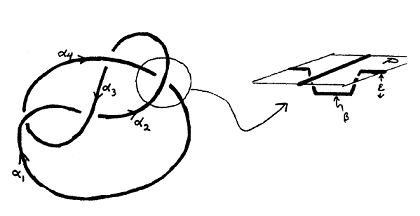
\includegraphics{knotdiagram.png}
	\caption \textbf{Construction of the diagram for the figure-eight knot. (Rolfsen)}
	\end{center}
\end{figure}


Given a classical knot $K \subset \mathbb{R}^3$, one may form a two-dimensional diagram by projecting the knot onto a plane and indicating the layering of the arcs at each crossing.  The diagram may then be used to go back to the three-dimensional knot, if desired.  Since $K$ is polygonal, we know that we can represent it using a finite number of arcs.  Divide $K$ into exactly enough arcs such that there are no intersections on the plane, and call them $\alpha_1, \alpha_2, \ldots, \alpha_n$.  Next one connects each of the $\alpha_j$ for $j = 1, 2, \ldots, n$ to $\alpha_{j-1}$ and $\alpha_{j+1}$, with these connections being made modulo $n$, with small arcs that go slightly below the plane.  Lastly, assign the arcs orientations that respect the ordering of their subscripts.  This is fairly hard to describe in words, but (Rolfsen) provides an excellent example, shown above in Figure 1.  The zoomed in portion on the right details the construction at the intersections.  The small arc under the plane is denoted $\beta$; it's some arbitrarily small distance below the plane $P$, denoted $\epsilon$.  The $x_i$ arrows are for the computation of the group of the knot, and can be ignored.
\\
\\
These diagrams are highly useful, and it turns out they can be created for any arbitrary polygonal knot.  
\\
\\
\textbf{Definition 8.} For a polygonal knot $K \subset \mathbb{R}^3$ and any plane $P$ along with its orthogonal projection $p: \mathbb{R}^3 \rightarrow P$, $P$ is \underline{regular} with respect to $K$ if for any $x \in P$, its preimage $p^{-1}(x)$ has an intersection with $K$ of at most two points.  If the intersection consists of two points, they cannot be a vertex of $K$ ($K$ is just a union of line segments).
\\
\\ Making note of the following three facts concerning an arbitrary polygonal knot $K$ and plane $P$, it becomes clear that a diagram may always be made:
\begin{itemize}
	\item It only takes arbitrarily minute perturbations of $P$ or $K$ to ensure $P$ to be regular for $K$.
	\item Denote the vertices of $K$ as $v_0, \ldots, v_r$.  For each knot $\exists \epsilon \in \mathbb{R}$ such that if one takes 			points $v_0', \ldots, v_r' \in \mathbb{R}^3$ with $|v_i - v_i'| < \epsilon$ for $i = 1, \ldots, r$, the polygon formed by these 			chosen points $K' = v_0' v_1' \ldots v_r' v_0'$ is a knot which is ambient isotopic to $K$.
	\item $K$ is ambient isotopic to the knot projection previously explained when $P$ is regular for $K$.
\end{itemize}
The idea is one can perturb $K$ to be regular for $P$ making adjustments small enough so that the resultant knot is ambient isotopic to $K$, then the projection will be an ambient isotopy.  The condition that if $p^{-1}(x)$ for some $x$ has two points then neither can be a vertex is necessary, for upon projecting down a vertex over an arc it would result in an erroneous intersection.  When there are two vertices in the preimage, the resulting intersection would have more than three arcs.
\\
\\
\subsection{Reidemeister Moves}
It's obvious given the limited nature of projecting three dimensional objects onto a plane that there will be ambiguities inherent to knot diagrams.  In particular, it's impossible in the general case to be certain when two diagrams actually represent the same knot. For example, the figure-eight knot appearing in Figure 1 has the following three differing diagrams:
\begin{figure}[htb!]
	\begin{center}
	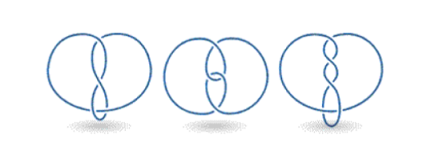
\includegraphics{figure8.png}
	\caption \textbf{Diagrams of the figure-eight knot (Adams)}
	\end{center}
\end{figure}

\noindent A case where it's possible to determine when two diagrams represent the same knot is when they both may be obtained from the
other using a finite sequence of three distinct moves, which are:

\begin{figure}[h!]
	\begin{center}
	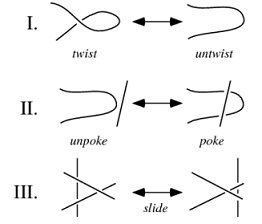
\includegraphics{moves.png}
	\caption \textbf{The three Reidemeister moves (Aneziris)}
	\end{center}
\end{figure} 
\clearpage

\noindent
\textbf{Theorem 9.}  Two diagrams represent knots which are ambient isotopic if and only if there exists a finite sequence of intermediary diagrams going from one to the other, where each diagram is obtained using exactly one Reidemeister move on the previous in the sequence.
\\

\noindent It's interesting to note that the numbering for the types corresponds to how many arcs are involved.  Many important invariants are actually defined using this concept.  In addition, it's extremely useful for checking for knot invariants using only diagrams.  One needs only check that no single Reidemeister move alters the alleged invariant.

\subsection{Seifert Surfaces}
Another useful construction associated with knots are Seifert surfaces, which are essentially just surfaces created by "filling in" the holes formed by the embedding in the larger space.  To formalize this notion, several definitions are required:
\\
\\
\textbf{Definition 10.} An n-dimensional \underline{manifold} $M^n$ is a metric space that can be covered with open sets that are homeomorphic to either $\mathbb{R}^n$ or $\mathbb{R}^n_+$.  $\mathbb{R}^n_+$ is the half space of $\mathbb{R}^n$ obtained by restricting one of the components to be strictly nonnegative: $\mathbb{R}^n_+ = \left\{{(x_1, x_2, \ldots, x_n) \in \mathbb{R}^n : x_n \ge 0}\right\}$. Points in $M$ that possess neighborhoods homeomorphic to $\mathbb{R}^n$ make up the \underline{interior} of $M$ which is denoted $\mathring{M}$.  The \underline{boundary} of $M$ is defined as $\partial M = M - \mathring{M}$. One calls a manifold closed if it's compact with $\partial M = \emptyset$ and open if $\partial M = \emptyset$ but it isn't compact.
\\
\\
\textbf{Definition 11.} A closed connected n-manifold $M$ is called \underline{orientable} when $H_n(M) \neq 0$.  When $\partial M \neq \emptyset$, it's called orientable if $H_n(M, \partial M) \neq 0$.
\\
\\
\textbf{Definition 12.} A subset $X \subset Y$ is \underline{bicollared} when there's an embedding \\ $b: X \times [-1,1] \rightarrow Y$ with $b(x,0) = x$, $\forall x \in X$.  Similarly to knots, the map $b$ itself or the embedding may referred to as the bicollar.  When $X^{n-1}$ and $Y^n$ are manifolds without boundary the bicollar is actually a neighborhood of $X$ in $Y$.

\begin{figure}[h!]
	\begin{center}
	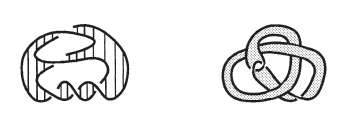
\includegraphics{seifert.png}
	\caption \textbf{Two Seifert surfaces (Lickorish)}
	\end{center}
\end{figure}

\noindent \textbf{Definition 13.} For some knot or link $K^n \subset S^{n+2}$, any connected, bicollared, and compact manifold $M^{n+1} \subset S^{n+2}$ with $\partial M = K$ is called a \underline{Seifert surface}.
\\
\\ 
Seifert surfaces will be used later to construct cyclic coverings of knot complements.  In this case, homology proves to be a very valuable tool, which is quite opposite to the homology of the complements themselves.  The final item to consider for now is the cases where Seifert surfaces may be formed. It turns out:
\\
\\
\textbf{Theorem 13.} Any polygonal knot or link in $\mathbb{R}^3$ or $S^3$ has a corresponding polygonal Seifert surface.
\\
\\
\textbf{Proof:} (Rolfsen) Let $L \subset \mathbb{R}^3$ be some knot or link.  Perform a regular projection of $L$ onto some plane $P$, taking care to give each component an orientation.  Remove the overcrossing and undercrossing arcs at each intersection and replace them with "short cut" arcs in P as shown below.  The arcs must respect the orientations originally assigned. 

\begin{figure}[h!]
	\begin{center}
	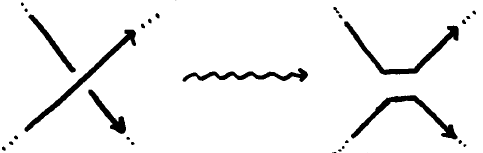
\includegraphics{shortcut.png}
	\caption \textbf{Creating closed arcs during Seifert surface construction.}
	\end{center}
\end{figure}

This leaves a disjoint collection of simple closed oriented arcs in $P$, with each bounding a disk with a bicollar.  These disks may overlap, but one only needs to push them slightly off the plane one by one so that they're disjoint.  Since they have bicollars, one can prescribe orientations labelling one side of each disk with a "+" and the other with a "-".  This assignment is arbitrary, but convention is such that the oriented boundary runs counterclockwise from the "+" side.  Next the disks are connected at the initial intersections with half-twisted strips which yields a single 2-manifold $M$ which clearly has $\partial M = L$. This step is visualized below.  When $L$ is just a knot, $M$ will be connected.  Otherwise, the last step is to join up the disjoint components of $M$ with tubes so that it's connected.  This proof is for the 3-dimensional case, but the theorem can actually be generalized to higher dimensions.  But first, another definition is necessary.
\clearpage
\begin{figure}[h!]
	\begin{center}
	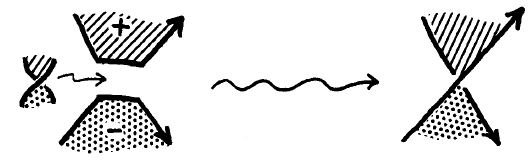
\includegraphics{strips.png}
	\caption \textbf{Connecting the disjoint disks}
	\end{center}
\end{figure}  

\textbf{Definition 14.} For any submanifold $M^m \subset N^n$ with $\partial M = \partial N = \emptyset$, the \underline{tubular neighborhood} of $M$ is an embedding $t: M \times B^{n-m} \rightarrow N$ with $t(x,0) = x$ $\forall x \in M$.  A submanifold is any subset of a manifold that is itself a manifold.
\\
\\
\textbf{Theorem 15.} Any polygonal knot or link $L^n \subset S^{n+2}$ that has a tubular neighborhood has a corresponding Seifert surface.
\\
\\
This theorem is merely stated.  The proof is quite in depth and doesn't have much to offer for the current study. 



























































\clearpage
\section{References}
Aneziris, C. N. "The Equivalence Moves." Ch. 4 in The Mystery of Knots: Computer Programming for Knot Tabulation. Singapore: World Scientific, pp. 29-33, 1999. 
\\
\\
Adams,  Colin  C.
The Knot Book: An Elementary Introduction to the
Mathematical Theory of Knots.
W. H. Freeman and Company, New York,
New York, 2001.


\end{document}